\documentclass[11pt, oneside, letterpaper]{article}
\usepackage{graphicx}
\usepackage{enumerate}
\usepackage{amsmath}
\usepackage{amssymb}
\usepackage[cm]{fullpage}
\RequirePackage[T1]{fontenc}
\RequirePackage{times}
\RequirePackage{charter} % Default font
\newcommand{\tasksep}{\noindent\underline{\hspace{\textwidth}}}
\providecommand{\figref}[1]{Fig.~\ref{#1}}

\begin{document}

\title{\huge\textbf{Perception in Robotics \\  Term 3, 2023. PS2}}
\author{Gonzalo Ferrer\\Skoltech}
\date{09 February 2023}
\maketitle


This problem set has a single task, comprising 15\% of your course grade, which is individual work. You are encouraged to talk at the conceptual level with other students, discuss on the equations and even on results, but you may not show/share/copy any non-trivial code.



\section*{Submission Instructions}
Your assignment must be received by 11:59pm on Tuesday, February 22nd.  You are to upload your assignment directly to the Canvas website as two attachments:
\begin{enumerate}
\item A \texttt{.tgz} or \texttt{.zip} file \textit{containing a directory} named after your uniqname with the structure shown below.

  \texttt{alincoln\_ps2.tgz}:\\
  (these are the files from the starting code. You should not modify them.)\\
  \texttt{alincoln\_ps2/run.py}\\
  \texttt{alincoln\_ps2/field\_map.py}\\
  $\ldots$ \\
  (plus those files that you have modified, i.e. filters or any other auxiliary file used)\\
  \texttt{alincoln\_ps2/filters/ekf.py}\\
  \texttt{alincoln\_ps2/filters/pf.py}\\
  \texttt{alincoln\_ps2/video\_ekf.\{avi,mp4\}}\\
  \texttt{alincoln\_ps2/video\_pf.\{avi,mp4\}}

\item A PDF with the written portion of your document, solving the tasks proposed below. Scanned versions of   hand-written documents, converted to PDFs, are perfectly acceptable.  No   other formats (e.g., .doc) are acceptable.  Your PDF file should adhere to  the following naming convention: \texttt{alincoln\_ps2.pdf}.

\end{enumerate}

Homework received after 11:59pm is considered late and will be penalized as per the course policy. The ultimate timestamp authority is the one assigned to your upload by Canvas.  No exceptions to this policy will be made.


\section*{Task 1: Landmark localization}

The key goal of this exercise is to get an understanding of the properties of Extended Kalman Filters (EKFs) and Particle Filters (PFs) for state estimation. You should try to ``play around'' with the parameters of each algorithm, so as to see how they deal with different levels of noise.

For this task, you will be implementing landmark-based robot localization (\figref{F:robosoccer}) using an EKF and PF with known data association. Essentially, your job is to replicate the results shown in figures 7.11 and 8.12 in the ProbRob text.
\begin{figure}[h]%
  \centering%
  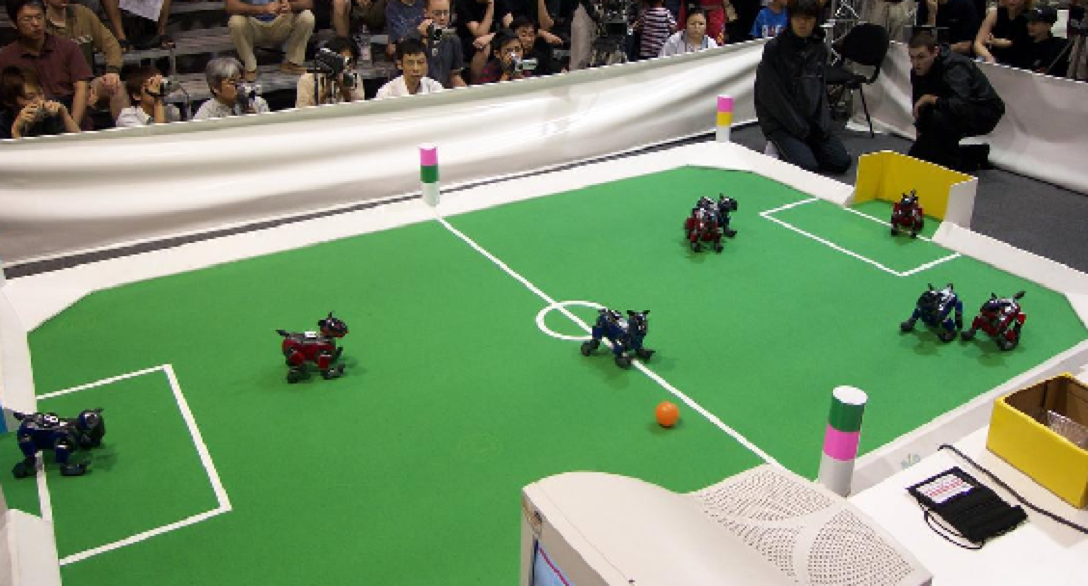
\includegraphics[width=0.65\textwidth]{./figures/specs/robosoccer.png}%
  \caption{Beacon-based robot localization.}%
  \label{F:robosoccer}%
\end{figure}


\subsection*{Code}
To begin, you will need to pull from the class repository to get the latest version.  This directory file contains a collection of python files that replicate the landmark-based planar localization simulation used in Chapters~7 and 8 of the ProbRob text.  Below you will find descriptions of the files included in the \texttt{.zip} file. You may end up not using every single file. Some are utilities for other files, and you don't really need to bother with them. Some have useful utilities, so you won't have to reinvent the wheel. Some have fuller descriptions in the files themselves.\\
\emph{Things to implement.} Each of these filters is based on the base class \texttt{LocalizationFilter} 
\begin{itemize}
\item \texttt{ekf.py} -- EKF
\item \texttt{pf.py} -- PF
\end{itemize}
\emph{Utilities} (you should not need to modify these files)
\begin{itemize}
\item \texttt{README.md} -- Some commands examples for installing the environment, testing and evaluating the task.
\item \texttt{run.py} -- Main routine, with multiple options, allowing you to solve the task with no need to modify the file.
\item \texttt{field\_map.py} -- for plotting the map.
\item \texttt{tools/task.py} -- General utilities available to the filter and internal functions.
\item \texttt{tools/data.py} -- Routines for generating, loading and saving data.
\item \texttt{tools/objects.py} -- Data structures for the project.
\item \texttt{tools/plot.py} -- All utilities for plotting data.
\item \texttt{filter/localization\_filter.py} -- An abstract base class to implement the various localization filters.
\end{itemize}


\subsection*{Data Format}
\begin{itemize}
\item State: $[x,y, \theta]$; (cm, cm, radians)
\item Observation: [bearing to landmark, landmark ID]; (radians, integer)
\item Motion Control: $[\delta_{\text{rot1}},\delta_{\text{trans}},\delta_{\text{rot2}}]$; (radians, cm, radians)
\end{itemize}

\begin{figure}[h]%
	\centering%
	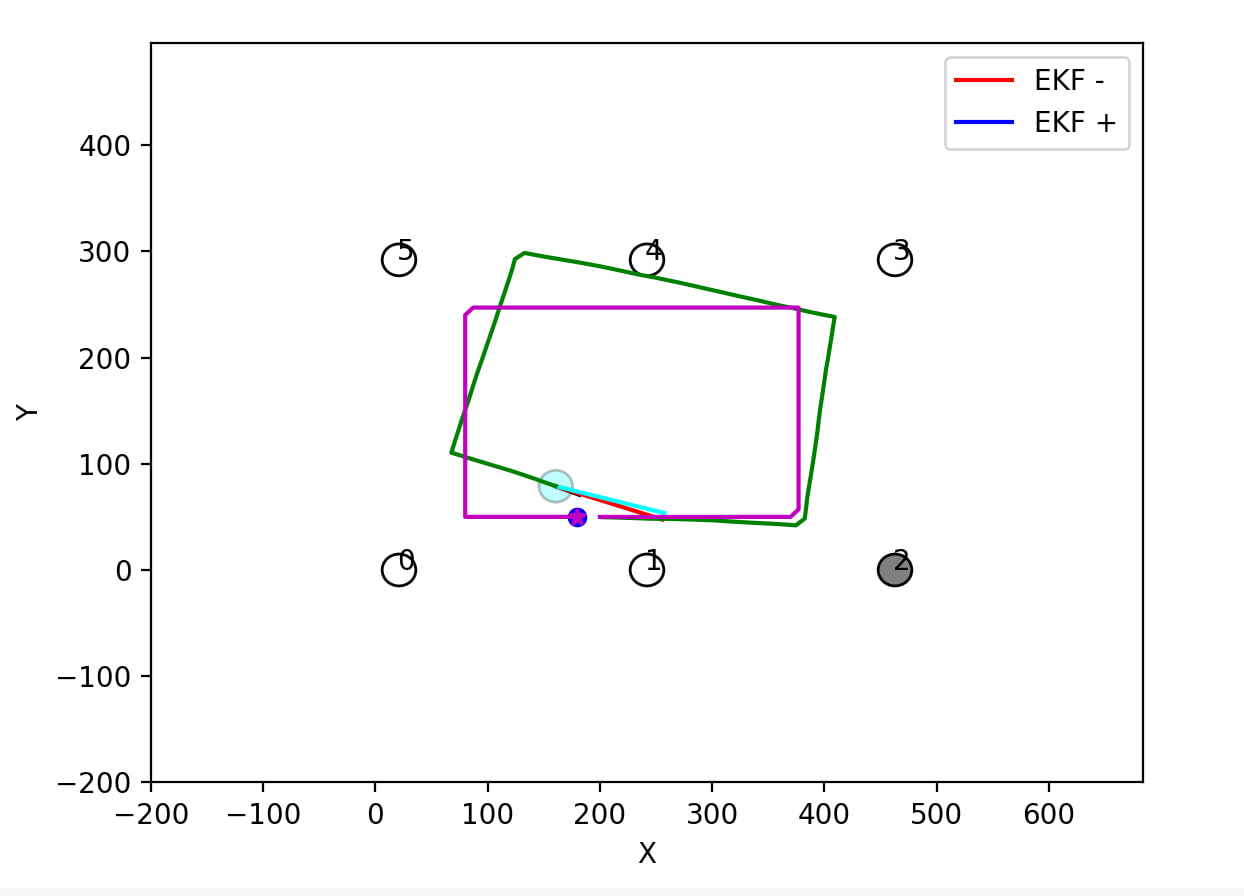
\includegraphics[width=0.65\textwidth]{./figures/specs/simulator_no_filter.png}%
	\caption{Simulator without filter-based solution.}%
	\label{F:simulator_no_filter}%
\end{figure}


\begin{figure}[h]%
  \centering%
  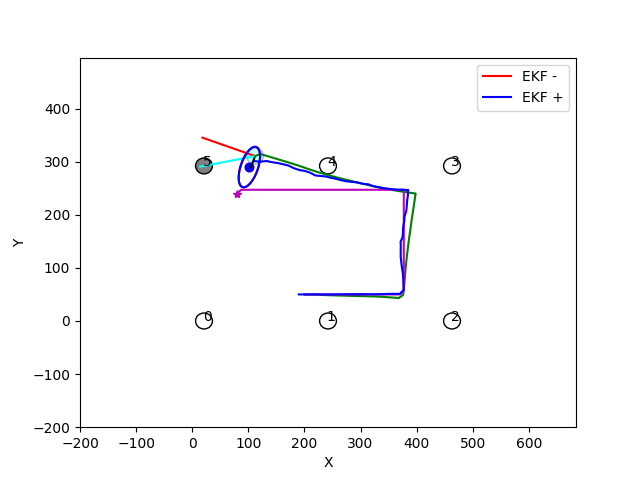
\includegraphics[width=0.65\textwidth]{./figures/specs/simulator.png}%
  \caption{Simulator with filter-based solution.}%
  \label{F:simulator}%
\end{figure}

\subsection*{Instructions}

The project generates motion information according to the odometry-based motion model of Chapter~5. Observations are landmark detections sensed through noisy bearing measurements. Each landmark has a unique ID and so data association is \textit{known} for this exercise.Unless you implement a filter-based solution, calling \texttt{python run.py -\,-animate -s} will generate a random simulation of 100 time steps see \figref{F:simulator_no_filter}. After implementing a solution you should obtain a picture as \figref{F:simulator}. Below is the description of plots:
\begin{enumerate}
\item The numbered circles represent landmarks 1 thru 6.  The circle colored in gray is the   landmark currently being observed.
\item The light blue circle represents the current robot pose---orientation is depicted by the black bar.
\item The magenta path is the ideal trajectory of the robot if there was no noise in the transition function. This is where the robot would ``think'' it is based upon the commanded odometry sequence only.
\item The green path is the actual trajectory of the robot---this state is   hidden to the filter and is known only to the simulation.  This is the   actual path that the robot took because of noise affecting the transition function.
\item The blue line is the filtered trajectory given the noisy actions and observations. It is the filter's job to provide updates on the position as accurate as possible.
\item The cyan line is the true, noise-free, landmark bearing observation,   which is unavailable to the filter.
\item The red line is the noise corrupted landmark bearing \texttt{observation} variable, this is available to the filter.
\end{enumerate}

If you run the simulation without specifying any input file, then a simulated trajectory of n = 100 time-steps will be generated: \texttt{python run.py -\,-animate -s -f ekf -n 100}. Here you should specify which filter \{ekf, pf\} you want to use.
Your job is to write a PF and EKF for robot localization at the corresponding folder \texttt{filters} and \texttt{run.py} will take care of calling those functions. 
For the evaluation of this exercise, the project folder contains a data file named \texttt{evaluation-input.npy} which would be common for everyone and it {\bf will be used to evaluate your solution}. To run a given data file, execute: \texttt{python run.py -\,-animate -s -f ekf -i evaluation-input.npy -o out} and outputs the result of your filter (necessary for task C).

In order to get quantitative results, you should generate plots that show the different evaluation criteria on the abscissa, and the corresponding filter error on the ordinate. For instance, you can plot number of samples versus average localization error, where error is measured by the distance between the true robot position and the estimate. In particular, generate the following plots, which should be included in your submitted report:

\begin{enumerate}[A.]
%TODO specify Q how looses dimensionality. SOmewhere it was incorrectly explained!!!
\item (15 pts) %Before implementing anything it is always a good practice to think on the problem.
  Before implementing anything, take a look at the code and answer the following questions.
  Write the value for the covariance  $Q$ of the noise added to the observation function, knowing that the parameter \texttt{bearing\_std} is its standard deviation. To find out which is the value of \texttt{bearing\_std} you should look at the default parameters passed to \texttt{run.py} lines 44 - 121.
 Write the equation for the covariance  $R_t$ of the noise added to the transition function, as explained in class
  and their corresponding numeric values for the initial robot command $u = [\delta_{rot1}, \delta_{trans}, \delta_{rot2}]^\top = [0, 10, 0]^\top$. Find out the default values of $\alpha$ in \texttt{run.py} line 152.
  Then derive the equations for the Jacobians $G_t$, $V_t$ and $H_t$, and evaluate them at the initial mean state
  $\mu_1 = [x,y,\theta]^\top = [180, 50, 0]^\top$ as it is considered in \texttt{run.py}. (It is not requested to evaluate observation Jacobians.)
\item (50 pts) Implement EKF and PF-based robot localization using odometry and bearing-only observations to features in a landmark map.
Remember to run the evaluation command to properly use the common created data file \texttt{evaluation-input.npy}.
  \begin{enumerate}[1.]
  \item For the EKF plot the filter estimated mean position and     3-sigma covariance ellipsoid overlaid on top of the simulation figure at     every time step.  If your filter is working correctly, the robot should     lie within the 3-sigma ellipse 98.89\% of the time.
  \item For the PF, plot the sample distribution every time step, it should be     centered on the robot's true position.
  \end{enumerate}

  Include videos in your submission for the EKF and PF under evaluation  conditions  and  using the corresponding input parameter -m.

\item (20 pts) Create plots of pose error versus time i.e., a plot of   $\hat{x}-x$ vs. $t$, $\hat{y}-y$ vs $t$, and $\hat{\theta}-\theta$ vs. $t$   where $(\hat{x},\hat{y},\hat{\theta})$ is the filter estimated pose and   $(x,y,\theta)$ is the ground-truth actual pose known only to the simulator.   Plot the error in blue and in red plot the $\pm 3\sigma$ uncertainty bounds.   Your state error should lie within these bounds approximately $99.73\%$ of   the time (assuming Gaussian statistics).  For the PF, use the sample mean   and variance.


\item (15 pts) Once your filters are implemented, please investigate some   properties of them. How do they behave
  \begin{itemize}
  \item as the sensor or motion noise go toward zero? (Please provide plots and explanation)
  \item as the number of particles decrease?
  \item if the filter noise parameters underestimate or overestimate the true noise parameters? Please clarify what underestimation and overestimation of noise is?
  \end{itemize}
(Items 1 and 3 are for EKF and "the noise" refers to both observation and control noises)
%\item(5 pts): Try to see how the algorithms handle global localization and the kidnapped robot problem using the Particle Filter.

\end{enumerate}


\end{document}
